\documentclass[orivec]{llncs}
\usepackage{graphicx}
\usepackage{amsmath}			% for "cases"
\usepackage{amsfonts}		% for frakur fonts
\usepackage{mathrsfs}		% for curly "E" error symbol
\usepackage{float}
\usepackage{tcolorbox}		% for wrapping example in color box
\usepackage{wrapfig}			% wrap figure beside text, used in example
\usepackage{tikz-cd}			% commutative diagrams
\usepackage{amssymb}			% for \multimap, \updownarrow, \bigstar
\usepackage{sectsty}			% change section color
\usepackage{turnstile}		% longer turnstiles

\usepackage{geometry}		% change paper size
\geometry{
  a4paper,         % or letterpaper
  textwidth=18cm,  % llncs has 12.2cm
  textheight=27cm, % llncs has 19.3cm
  heightrounded,   % integer number of lines
  hratio=1:1,      % horizontally centered
  vratio=2:3,      % not vertically centered
}
\usepackage[fontsize=13pt]{scrextend}

\ifdefined\chinchin
\usepackage{xeCJK}
\setCJKmainfont[BoldFont=SimHei,ItalicFont=KaiTi]{SimSun}
\newcommand{\cc}[2]{#1}
\else
\newcommand{\cc}[2]{#2}
\fi

% *************** Delete when not using colors **********************
\usepackage{color}
\definecolor{Cerulean}{RGB}{100,100,200}
\newcommand{\emp}[1]{\textbf{\textcolor{Cerulean}{#1}}}
\definecolor{grey}{rgb}{0.9,0.9,0.9}  % grey

% \chapterfont{\color{blue}}  % sets colour of chapters
\sectionfont{\color{blue}} 
\subsectionfont{\color{blue}} 
\subsubsectionfont{\color{blue}} 

\newcommand{\vect}[1]{\boldsymbol{#1}}
\newcommand*\sigmoid{\vcenter{\hbox{
\includegraphics{sigmoid.png}}}}
\newcommand*\KB{\vcenter{\hbox{
\includegraphics{KB-symbol.png}}}}
\newcommand*\invsigmoid{\vcenter{\hbox{
\includegraphics{inverse-sigmoid.png}}}}
\newcommand{\invW}{\, \rotatebox[origin=c]{90}{W}}
\newcommand{\invw}{\, \rotatebox[origin=c]{90}{w}}
\newcommand*\rectifier{\vcenter{\hbox{
\includegraphics{rectifier.png}}}}
\newcommand{\dashh}{\textemdash~}

% ***** Boxed variables inside math equations
% \newcommand*{\boxedcolor}{black}
\makeatletter
% \renewcommand{\boxed}[1]{\textcolor{\boxedcolor}{%
% \fbox{\normalcolor\m@th$\displaystyle#1$}}}
% \setlength{\fboxsep}{1pt}
\renewcommand{\boxed}[1]{\fbox{\m@th$\displaystyle\scalebox{0.9}{#1}$} \,}
\makeatother

\overfullrule=0mm

\newsavebox{\MyName}
\savebox{\MyName}{
\includegraphics[scale=0.6]{YKY.png}}

\title{\cc{Jacobian 神经网络算法}{Jacobian neural network learning algorithm}}
\titlerunning{\cc{Jacobian 神经网络算法}{Jacobian NN learning algorithm}}
\author{\usebox{\MyName} (King-Yin Yan)
% \\ \footnotesize{General.Intelligence@Gmail.com}
}
\institute{General.Intelligence@Gmail.com}

\begin{document}

\maketitle
\setlength{\parindent}{0em}
% \setlength{\parskip}{2.8ex plus0.8ex minus0.8ex}
\setlength{\parskip}{2.8ex}

\cc{
经典的神经网络 Back Prop 学习算法,它是一个 error-driven 算法,但在很多人工智能的实际应用中,不存在唯一的「理想答案」,而是根据正或负的奖励 (reward) 学习。  当答案正确时,奖励 $> 0, \mbox{error} = 0$; 当答案不正确时,奖励 $< 0$,但 $\mbox{error}$ 仍是不知道的(因为不知道理想答案)。  简言之,就是不能用 error-driven 学习。 
}{
The classical Back Prop algorithm is \textbf{error-driven}, but in many AI problems the ``correct'' answers are not given, instead the feedback is provided via \textbf{rewards}. When an answer is correct, the reward $R > 0$, error $\mathscr{E} = 0$; when the answer is incorrect, $R < 0$, but $\mathscr{E}$ is still unknown (because we don't know the correct answer).  In other words, error-driven learning is inapplicable.
}

\cc{
所以我想出了一个 reward-driven 的学习法: 假设神经网络将 $\vect{x}_0 \mapsto \vect{y}_0$,它通常也会将 $\vect{x}_0$ 的邻域 map 到 $\vect{y}_0$ 的邻域。 如果我们想「加强」这个映射,可以将「更大的 $\vect{x}_0$ 的邻域」映射到「接近 $\vect{y}_0$ 的邻域」。
}{
So I thought of a reward-driven learning method:  assume the neural network maps $\vect{x}_0 \mapsto \vect{y}_0$, usually it also maps the neighborhood of $\vect{x}_0$ to the neighborhood of $\vect{y}_0$.  If we wish to ``strengthen'' this pair of mapping, we can make a \textbf{bigger} neighborhood of $\vect{x}_0$ map to the same neighborhood close to $\vect{y}_0$.  We will make this precise.
}

\cc{
这种算法对人工智能应该很重要,暂时我还想不出有什么其他办法,可以做到[深度]神经网络的 reward-driven 学习。 
}{
This type of learning algorithm should be very useful to AI, and currently the author is not aware of other alternatives for training [deep] neural networks via rewards.
}

\cc{
将这思想更准确化,可以将 feed-forward 神经网络的构造看成是这样的:
}{
A feed-forward neural network can be constructed this way:
}
\begin{eqnarray}
\vect{y} &=& \vect{F}(\vect{x}) \\
\vect{y} &=& \sigmoid \stackrel{_L}{W} ... \sigmoid \stackrel{_\ell}{W} ... \sigmoid \stackrel{_1}{W} \vect{x}
\end{eqnarray}
\cc{
其中 $W$ 代表每一层 (layer) $\ell$ 的矩阵。
}{
where $W$ represents the matrix of \textbf{weights} on each layer $\ell$.
}

\cc{
(下面会用到)$F$ 的\textbf{反方向}是:
}{
(We shall use this later) The \textbf{inverse} of $F$ is:
}
\begin{eqnarray}
\vect{x} &=& \vect{F}^{-1}(\vect{y}) \\
\vect{x} &=& \stackrel{_1}{\invW} \invsigmoid ... \stackrel{_\ell}{\invW} \invsigmoid ... \stackrel{_L}{\invW} \invsigmoid \; \vect{y}
\end{eqnarray}
\cc{
注意: $\invW = W^{-1} \;,\; \invsigmoid = \sigmoid^{-1}$,形状不同。
}{
Note: $\invW = W^{-1} \;,\; \invsigmoid = \sigmoid^{-1}$, the shape is different.
}

\cc{
假设在 $\vect{x}$ 空间有体积元 $U$,经过 $\vect{F}$ 变换成 $\vect{y}$ 空间的体积元 $V$,那么:
}{
Assume that in the space of $\vect{x}$ there is a volume element $U$, which transforms via $\vect{F}$ to a volume element $V$ in the space of $\vect{y}$, then:
}
\begin{equation}
U = |J| \cdot V
\end{equation}
\cc{
$\displaystyle J = \left[ \frac{\partial \vect{F}(x)}{\partial x} \right]$ 叫 Jacobian 矩阵。
}{
$\displaystyle J = \left[ \frac{\partial \vect{F}(x)}{\partial x} \right]$ is called the \textbf{Jacobian} matrix.
}

\cc{
在我们的情况下,$\displaystyle |J| = \left| \frac{\partial \vect{F}^{-1}(\vect{y})}{\partial \vect{y}} \right|$ 在 $\vect{y}_0$ 的值,代表「单位体积元由 $\vect{y}_0 \mapsto \vect{x}_0$ 的变化率」。 (下面会看到,$\vect{F}$ 和 $\vect{F}^{-1}$ 的正/反方向不太重要,因为基本上不影响计算复杂度。)
}{
In our case, the value of $\displaystyle |J| = \left| \frac{\partial \vect{F}^{-1}(\vect{y})}{\partial \vect{y}} \right|$ at $\vect{y}_0$ represents ``the change in volume from $\vect{y}_0 \mapsto \vect{x}_0$''.  (Below, we will see that the direction of $\vect{F}$ or $\vect{F}^{-1}$ is not too important, as either way the computational complexity is essentially the same.)
}
\begin{equation}
\vcenter{\hbox{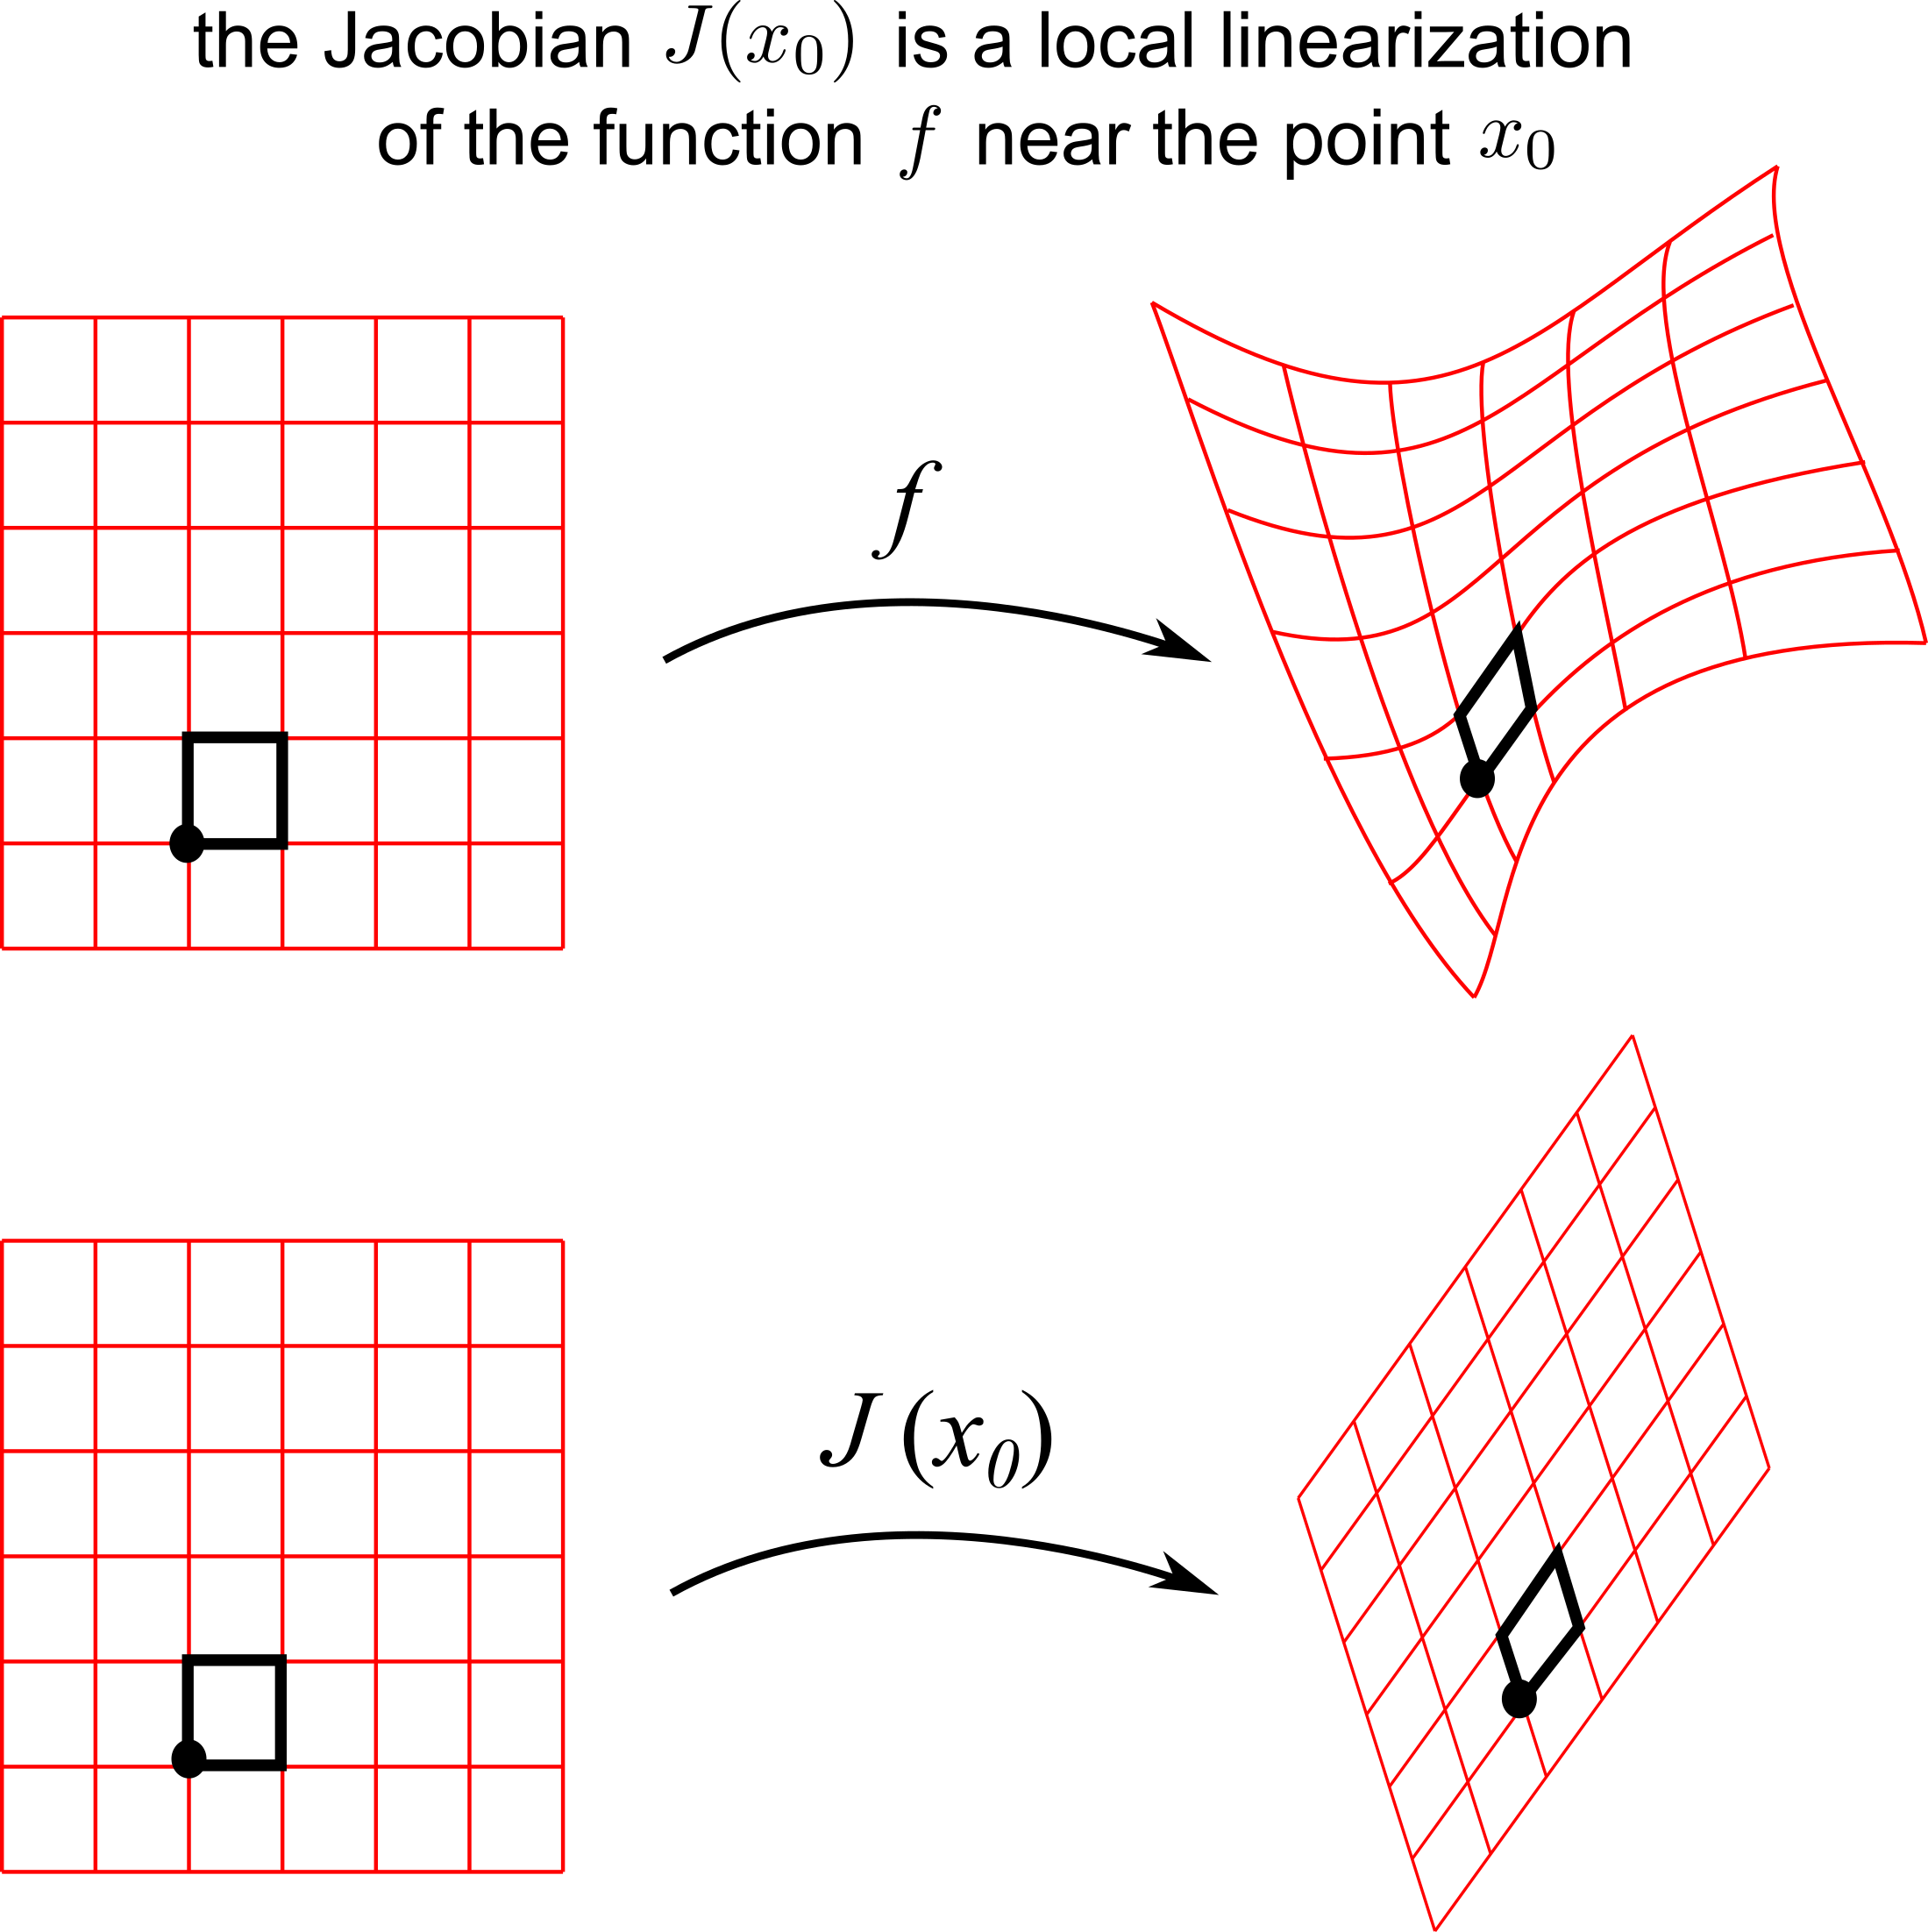
\includegraphics[scale=0.7]{Jacobian.png}}}
\end{equation}

\cc{
每次得到\textbf{正奖励},我们会令 Jacobian $|J|$ 增加一点:
}{
Every time we get a \textbf{positive reward}, we can let the Jacobian $|J|$ increase slightly:
}
\begin{equation}
|J| := \det \left[ \frac{\partial \vect{F}^{-1}(\vect{y})}{\partial \vect{y}} \right]_{n \times n}
\end{equation}
\cc{
下标表示那是一个 $n \times n$ 矩阵。
}{
The subscript indicates that it is a $n \times n$ matrix.
}

\cc{
其实 Jacobian 矩阵的意义就是:
\begin{equation}
J = \left[ \frac{\partial \mbox{ 输出}}{\partial \mbox{ 输入}} \right]
\end{equation}
}{
The meaning of the Jacobian matrix is:
\begin{equation}
J = \left[ \frac{\partial \mbox{ input}}{\partial \mbox{ output}} \right]
\end{equation}
}
\cc{
神经网络的输入和输出都是 $\dim n$,所以 Jacobian 很自然是 $n \times n$ 矩阵。
}{
The neural network's input and output are both of $\dim n$, so the Jacobian is naturally an $n \times n$ matrix.
}

\cc{
用\textbf{梯度下降法},我们需要计算这些梯度: $\displaystyle \left[ \frac{\partial |J|}{\partial \vect{W}} \right]$,总数是网络中的 weights 的个数 $ = \sum m_\ell$。 
}{
To use \textbf{gradient descent}, we need to calculate these gradients: $\displaystyle \left[ \frac{\partial |J|}{\partial \vect{W}} \right]$, their total number is the number of weights in the network $= \sum \ell \; \#(\stackrel{_\ell}{W})$.
}

\cc{
要用到 determinant 的微分公式:
}{
We need the formula for the derivative of the determinant:
}
\begin{eqnarray}
\frac{d}{dt} |A(t)| = tr ( \mbox{adj}(A) \cdot \frac{dA(t)}{dt} ) \\
\mbox{adj}(A) := |A| \cdot A^{-1}
\end{eqnarray}
\cc{
换句话说,对於每个权重 $w := \stackrel{\ell}{W}_{ij}$,我们要计算:
}{
In other words, for each weight $w := \stackrel{\ell}{W}_{ij}$, we need to calculate:
}
\begin{equation}
\frac{\partial}{\partial w} |J| = tr ( |J| \cdot J^{-1} \cdot \left[ \frac{\partial J}{\partial w} \right] )
\end{equation}
\cc{
注意: $|J|$ 和 $J^{-1}$ 是 $\vect{y}_0$ 的函数,只需在大 loop 外一次过计算。
}{
Note: $|J|$ and $J^{-1}$ are functions of $\vect{y}_0$, we only need to calculate them once outside the big loop.
}

\cc{
问题是,计算 $\displaystyle \left[ \frac{\partial J}{\partial w} \right]_{n \times n}$ 的时候:
}{
Now a problem arises in the calculation of $\displaystyle \left[ \frac{\partial J}{\partial w} \right]_{n \times n}$:
}
\begin{equation}
\frac{\partial J}{\partial w} = \frac{\partial}{\partial w} \frac{\partial \vect{F}^{-1}}{\partial y} = \frac{\partial}{\partial w} \frac{\partial}{\partial \vect{y}} \; \stackrel{_1}{\invW} \invsigmoid ... \stackrel{_\ell}{\invW} \invsigmoid ... \stackrel{_L}{\invW} \invsigmoid \; \vect{y}
\end{equation}
\cc{
这牵涉到用 $w$ 对 $W^{-1}$ 的分量微分,可以想像就算计了出来也会是极复杂的。 解决办法是,索性「\textbf{本末倒置}」,用 $\invW$ 来定义神经网络,然后在 forward propagation 时才用 $W = \invW^{-1}$ 计算。
}{
This requires us to differentiation $W^{-1}$ w.r.t. $w$;  we can imagine the result would be very complicated.  So we use a trick, by ``reversing'' the network, we use $\invW$ to define the network weights, and then use $W = \invW^{-1}$ during forward propagation.
}

\cc{
$J$ 的分量写出来是:
}{
The components of $J$ are:
}
\begin{equation}
J_{ij} = \displaystyle \frac{\partial \vect{F}^{-1}_i}{\partial y_j} = \frac{\partial}{\partial y_j} \left[ \stackrel{_1}{\invW} \invsigmoid ... \stackrel{_\ell}{\invW} \invsigmoid ... \stackrel{_L}{\invW} \invsigmoid \; \vect{y} \right]_i =: \nabla^1_{i j} \\
\end{equation}
% & = \sum_{k_1} (\, \stackrel{_1 \hspace{15pt}}{\invW_{i k_1}} \invsigmoid' ... \sum_{k_\ell} (\, \stackrel{_\ell \hspace{21pt}}{\invW_{k_{\ell - 1} k_\ell}} \invsigmoid' ... \sum_{k_L} (\, \stackrel{_L \hspace{25pt}}{\invW_{k_{L - 1} k_L}} \invsigmoid' (y_{k_L}) \displaystyle \frac{\partial y_{k_L}}{\partial y_j} ))) \nonumber
\begin{equation}
\begin{cases}
\nabla^1_{i j} &:= \displaystyle \sum_{k_1} [\, \stackrel{_1 \hspace{11pt}}{\invW_{i k_1}} \invsigmoid'(y^2_{k_1}) \nabla^2_{i j} \,] \\
\nabla^\ell_{i j} &:= \displaystyle \sum_{k_\ell} [\, \stackrel{_\ell \hspace{22pt}}{\invW_{k_{\ell - 1} k_\ell}} \invsigmoid'(y^{\ell + 1}_{k_\ell}) \nabla^{\ell + 1}_{i j} \,] \\
\nabla^L_{i j} &:= \quad \quad \displaystyle \stackrel{_L \hspace{21pt}}{\invW_{k_{L - 1} j}} \invsigmoid' (y_j)
\end{cases}
\end{equation}
\cc{
这情况完全类似於经典 Back Prop,以上只是 chain rule 的应用,$\nabla^\ell$ 将每层用 chain rule 分拆开来,所以 $\nabla$ 又叫 ``local gradient''。 上式就是整个网络的\textbf{反向传递},其中每个 weight 出现 exactly 一次。
}{
This situation is exactly analogous to the classical Back Prop algorithm;  The above is just the application of the \textbf{chain rule}, with $\nabla^\ell$ written separately for each layer, therefore $\nabla$ is called the ``local gradient''.  The above formula amounts to propagating the entire network one time, where every weight appears \textbf{exactly once}.
}
%但 $\displaystyle \frac{\partial y_{k_L}}{\partial y_j}$ 只有当 $k_L = j$ 时为 $1$,其他全为 $0$,所以前面各项没变,最后的一个 $\sum$ 改写:
%\begin{equation}
%J_{ij} = \sum_{k_1} (\, \stackrel{_1 \hspace{15pt}}{\invW_{i k_1}} \invsigmoid' ... \sum_{k_\ell} (\, \stackrel{_\ell \hspace{21pt}}{\invW_{k_{\ell - 1} k_\ell}} \invsigmoid' ...  \stackrel{_L \hspace{21pt}}{\invW_{k_{L - 1} j}} \invsigmoid' (y_j) \;))
%\end{equation}

\cc{
但工作还未完,我们要计算 $\displaystyle \frac{\partial J_{ij}}{\partial \invw} = \dot{\nabla}^1_{ij}$。 (定义 $\invw := \stackrel{\ell}{\invW}_{g h} \;,\; k_0 := i \;,\; k_L := j$) \\
注意: $\vect{x} = \vect{F}^{-1}(\vect{y})$,所以 $\vect{y}$ 是\textbf{自变量},$\invw$ 不影响 $\vect{y}$,所以 $\displaystyle \frac{\partial \vect{y}}{\partial \invw} \equiv 0$。\\
{\color{red}上面这句好像有问题: 搞不清是 who depends on whom,以下可能错误。} \\
%\frac{\partial J_{ij}}{\partial \invw} = \frac{\partial}{\partial \invw} \sum_{k_1} (\, \stackrel{_1 \hspace{15pt}}{\invW_{k_0 k_1}} \invsigmoid' ... \sum_{k_\ell} (\, \stackrel{_\ell \hspace{21pt}}{\invW_{k_{\ell - 1} k_\ell}} \invsigmoid' ...  \stackrel{_L \hspace{21pt}}{\invW_{k_{L - 1} k_L}} \invsigmoid' (y_j) \;))
$\invw$ 必会是 $\invW$ 的其中一元,但如果 $\invw \not\in \invW$,以下的项微分后都会变成 $0$:
}{
But our work is not finished yet;  We need to calculate $\displaystyle \frac{\partial J_{ij}}{\partial \invw} =: \dot{\nabla}^1_{ij}$. \\
(Let's define $\invw := \stackrel{\ell}{\invW}_{g h} \;,\; k_0 := i \;,\; k_L := j$) \\
Note: $\vect{x} = \vect{F}^{-1}(\vect{y})$, so $\vect{y}$ is the \textbf{independent variable}, $\invw$ does not influence $\vect{y}$, so $\displaystyle \frac{\partial \vect{y}}{\partial \invw} \equiv 0$. \\
{\color{red}There may be a problem here:  can't figure out who depends on whom, so what follows may be wrong.} \\
$\invw$ would be an element of $\invW$, but if $\invw \not\in \invW$, all the terms below would vanish:
}
\begin{equation}
\begin{cases}
\displaystyle \dot{\nabla}^1_{i j} = \sum_{k_1} \left[\, \stackrel{_1 \hspace{15pt}}{\invW_{i k_1}} \invsigmoid'(y^2_{k_1}) \dot{\nabla}^2_{i j}  \,\right] \\
\displaystyle \dot{\nabla}^\ell_{i j} = \sum_{k_\ell} \left[\, \stackrel{_\ell \hspace{15pt}}{\invW_{k_{\ell - 1} k_\ell}} \invsigmoid'(y^{\ell + 1}_{k_\ell}) \dot{\nabla}^{\ell + 1}_{i j} \,\right] \\
\displaystyle \dot{\nabla}^L_{i j} = \quad \quad \stackrel{_L \hspace{21pt}}{\invW_{k_{L - 1} j}} \invsigmoid' (y_j) \equiv 0
\end{cases}
\end{equation}
\cc{
所以实际上只剩下一项:
}{
So what is left over is just this term:
}
\begin{eqnarray}
& \displaystyle \frac{\partial J_{ij}}{\partial \invw} = \sum_{k_1} \left[\, \stackrel{_1 \hspace{15pt}}{\invW_{k_0 k_1}} \invsigmoid'(y^2_{k_1}) ... \sum_{k_{\ell - 2}} \left[\, \stackrel{_{\ell - 2} \hspace{27pt}}{\invW_{k_{\ell - 3} k_{\ell - 2}}} \invsigmoid'(y^{\ell - 1}_{k_{\ell - 2}}) ... \right. \right. \\
& \begin{cases}
... \; \left. \left. \stackrel{_{\ell - 1} \hspace{20pt}}{\invW_{k_{\ell - 2}, g}} \invsigmoid'(y^{\ell}_g) \, \invsigmoid'(y^{\ell + 1}_h) \nabla^{\ell + 1}_{i j} \right] \right] \\
... \; \left. \left. \stackrel{_{\ell - 1} \hspace{20pt}}{\invW_{k_{\ell - 2}, g}} \invsigmoid'(y^{\ell}_g) \, \invsigmoid'(y^{\ell + 1}_h) \right] \right] \quad \quad \quad \mbox{if } \invw \in \mbox{last layer} \nonumber
\end{cases}
\end{eqnarray}
% \sum_{k_{\ell + 1}} (\, \stackrel{_{\ell + 1} \hspace{21pt}}{\invW_{k_\ell k_{\ell + 1}}} \invsigmoid' ... \; \stackrel{_L \hspace{21pt}}{\invW_{k_{L - 1} k_L}} \invsigmoid' (y_j) \;)) \\
% &:=& \sum_{k_1} (\, \stackrel{_1 \hspace{15pt}}{\invW_{k_0 k_1}} \invsigmoid'' ... \; \invsigmoid' (\vect{u}) \;)
\cc{
上式的意思是: 每层 layer 重复一块 $\left[ \sum \invW \; \invsigmoid' \right]$,直到遇到 $\invw = \stackrel{\ell}\invW_{g h}$,则用结尾形式取代之。
}{
The above formula means:  For each layer we repeat a block of $\left[ \sum \invW \; \invsigmoid' \right]$, until we encounter $\invw = \stackrel{\ell}\invW_{g h}$, then we replace with the terminal form.
}

\cc{
和经典 Back Prop 不同的是,上式只是 $n \times n$ 矩阵中的一个元素,从复杂度而论,每个 weight 的 $\nabla$ 计算,增加了起码 $n^2$ 倍的复杂度(虽然其计算上可以共用一些结果)。 记住 $n = \mbox{dim } \boxed{\mbox{状态空间}}$。
}{
In contrast to classical Back Prop, the above formula gives us only one element in an $n \times n$ matrix;  From the complexity point of view, calculating the $\nabla$ for each weight is at least $n^2$ times as costly as classical Back Prop (even though we may re-use some intermediate computation results).  Recall that $n = \mbox{dim } \boxed{\mbox{state space}}$.
}

\cc{
可以这样理解: 每个 weight 的调教,需要计算这个 weight 对 Jacobian 的影响,而那 Jacobian 是\textbf{整个}网络的特性。 关键似乎就在於每个 weight 对 Jacobian 的\textbf{影响}。 
}{
We can understand it thusly:  For each weight we try to calculate its influence towards the Jacobian, but the Jacobian is a \textbf{global} property of the network.  The key seems to lie in how each weight \textbf{influences} the Jacobian.
}

\cc{
现在回看更高层次的这个式子:
}{
Now let's look back at this higher-level formula:
}
\begin{eqnarray}
\frac{\partial}{\partial w} |J| &=& tr ( |J| \cdot J^{-1} \cdot \left[ \frac{\partial J}{\partial w} \right] ) \\
&=& |J| \cdot tr ( \left[ \frac{\partial y}{\partial x} \right] \cdot \left[ \frac{\partial }{\partial w} \frac{\partial x}{\partial y} \right] ) \\
&=& |J| \cdot \sum_{i j} \left( \frac{\partial y}{\partial x} \right)_{i j} \left( \frac{\partial }{\partial w} \frac{\partial x}{\partial y} \right)_{i j}
\label{code-eqn}
\end{eqnarray}

\cc{
上式中最重要(最慢)的是那 $(i, j) \in n \times n$ 求和。 裡面的第一個因子是 Jacobian $J$,第二个因子是我们刚计算了的 $\nabla_w J^{-1}$。 
}{
The most critical (slowest) part is the $(i, j) \in n \times n$ summation.  The first factor inside $\sum$ is the Jacobian $J$, the second factor is the $\nabla_w J^{-1}$ that we just calculated. 
}

% 比较一下经典 Back Prop 算法: 对每个 weight 我们会计算 ``local gradient'' $\displaystyle \nabla = \frac{\partial \mbox{ 误差}}{\partial w}$,但那个 $\nabla$ 比较易计算。

\cc{
Back Prop 的 $\nabla$ 形式上是 $\displaystyle \frac{\partial \mbox{ 输出}}{\partial \, \mbox{w}}$,我们的 $\nabla$ 形式是 $\displaystyle \left[ \frac{\partial}{\partial w} \frac{\partial \mbox{ 输入}}{\partial \mbox{ 输出}} \right]_{n \times n}$。
}{
Back Prop's $\nabla$ has the form $\displaystyle \frac{\partial \, \boxed{\mbox{output}}}{\partial \, \boxed{\mbox{weights}}}$\\
whereas our $\nabla$ has the form $\displaystyle \left[ \frac{\partial}{\partial \, \boxed{\mbox{weights}}} \frac{\partial \, \boxed{\mbox{input}}}{\partial \, \boxed{\mbox{output}}} \right]_{n \times n}$.
}

\cc{
其实我们只需要计算 $\nabla_w |J|$ 的\textbf{大约方向}。 暂时我在代码中的做法是: 忽略式 (\ref{code-eqn}) 中较小的项,那就不需做足 $n^2$ 个乘积。 
}{
In fact we just need to calculate the \textbf{approximate} direction and size of $\nabla_w |J|$.  Currently in our code we use this trick:  ignore the smaller terms in (\ref{code-eqn2}), so we don't need to do all of $n^2$ products. 
}

\cc{
或者可不可以将 $|J|(\invw)$ 看成是一个 weight $\invw$ 的函数,然后用它的 Taylor series expansion 来近似? 
}{
Or perhaps we can regard $|J|(\invw)$ as a function of the weight $\invw$, and then use its Taylor series expansion to approximate?
}

\cc{
{\color{red}其实更大的问题是: 给定一个输入 $x$,整个 $F$ 只能输出一个值 ,因而不能做到 stochastic policy。 } 暂时搁置。
}{
{\color{red}Actually an even bigger problem is:  for a given input $x$, the entire $F$ can only output a single value $y$, so it cannot compute stochastic policies. }  So this idea is put on hold.
}


\begin{center}
\line(1,0){100} Notes \line(1,0){100}
\end{center}

\begin{itemize}
	\item Parameters are organized hierarchically (``deep'')
	\item Jacobian of $F$ at $x$ in terms of $W$ is easy to calculate
	\item 
\end{itemize}

%\begin{equation}
%\centering
%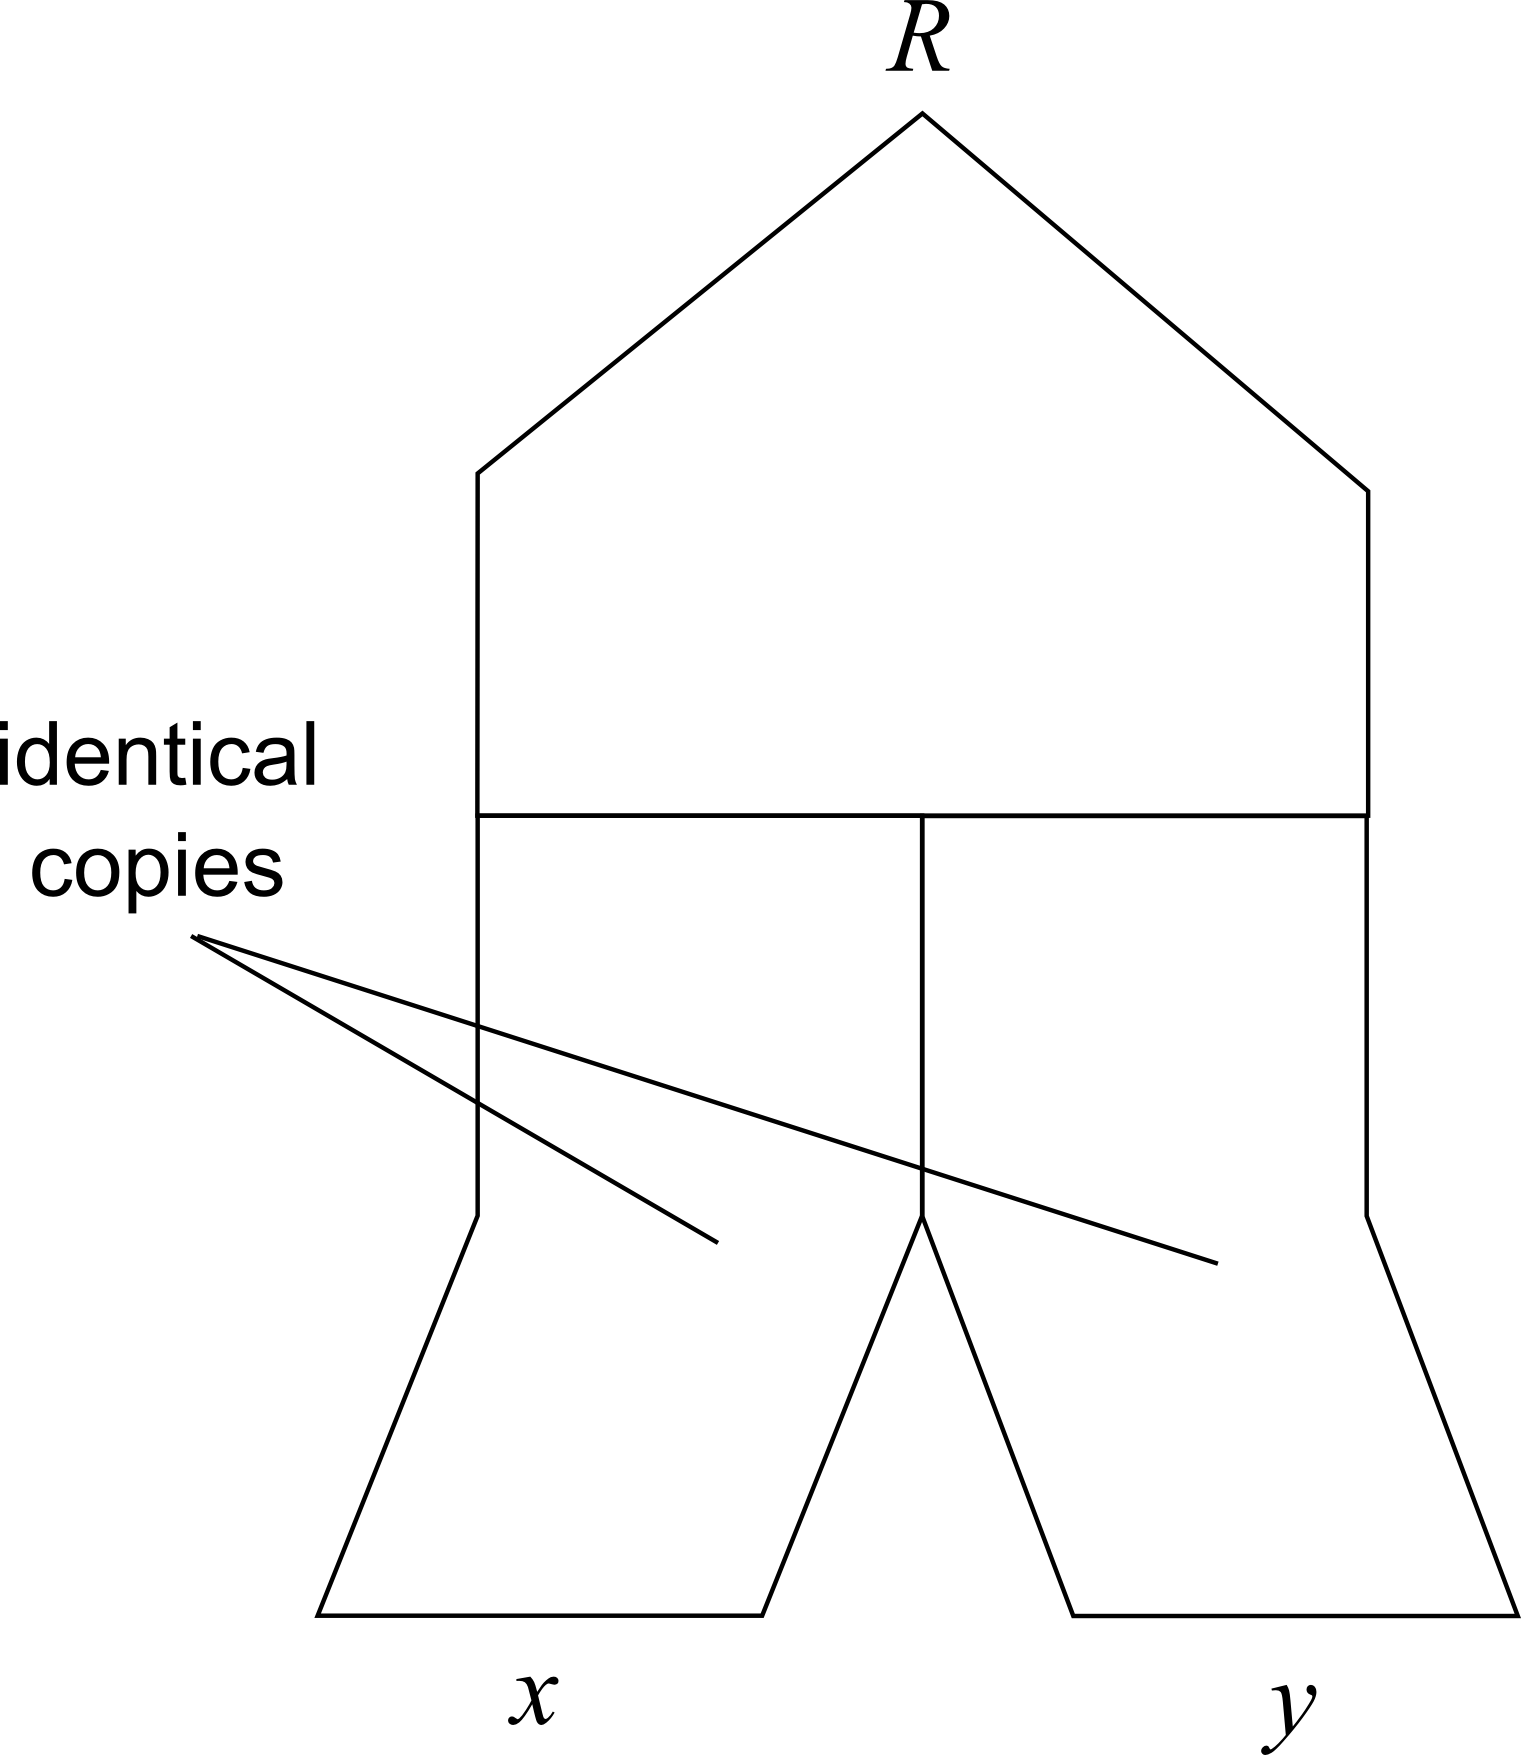
\includegraphics[scale=0.5]{R-network.png}
%\end{equation}

%或者,照旧是 feedforward network,但 somehow 它的学习是基於某 reward function。 问题是这 reward function 从何而来?  $R$ 可以是一个全部 $W$ 的函数,是由我们任意定义的。  

\bibliographystyle{plain} % or number or aaai ...
\bibliography{AGI-book}

\end{document}
